% =====================================================================
%  c04：原印刷页 31–38（PDF p.32–39）
%  唯一标题为 §2.2.7（\subsubsection 级）；片段自上一片段（c03）末尾
%  编号列表的第 2 项起排，故开头不补任何标题。
%  公式 (2.94)–(2.129) 连续；插图 2 幅（fig02、fig03）。
% =====================================================================

% [Tutor Note: 术语取舍：flat gauge field 译「平坦规范场」、flat connection 译「平坦联络」；holonomy function 译「和乐函数」，以强调它是圈空间上的函数（而不是单个和乐元素）；moduli stack 译「模叠」，与全书其余片段保持一致。]

% 原文 p.31 页首承接上一片段的编号列表（第 1 项在 c03 片段末尾），故此处从第 2 项起排。
\begin{enumerate}[start=2]
  \item 若改用 Maxwell-Chern-Simons 理论，情形就大不相同，因为作用量对时间导数是二阶的。规范场的正则共轭量是电场，但相空间上存在一个非平凡的、带联络的线丛。其中一部分内容在第 2.2.10 节中有解释。

  {\small\itshape ［原文标记：这里需要再多解释一些！］}% [原文待办标记，原文 p.31 右边栏]

  \item 下文我们将写下平坦联络的有限维模空间上显式的辛形式。在非阿贝尔情形，与相对简单的 Poisson 括号 (3.38) 不同，要在平坦联络的有限维模空间上显式写出辛结构绝非易事。

  {\small\itshape ［原文标记：这段议论大概应当放到非阿贝尔那一节，并且应当讨论 Goldman 括号等。］}% [原文待办标记，原文 p.31 右边栏]
\end{enumerate}

\subsubsection{曲面上的平坦规范场空间} % 原文: 2.2.7 The Space Of Flat Gauge Fields On A Surface

在我们对平坦规范场的模空间作几点评论之前，还需要一项预备工作。我们对路径排序指数（path-ordered exponential）的约定见附录 H。特别注意，$A$ 是 $\mathfrak{g}$ 中局部定义的形式，因而取值于反厄米矩阵。

{\small\itshape ［原文标记：这些约定也许需要改动：最好让相继的路径对应相继的右乘 $\mathrm{Pexp}$。］}% [原文待办标记，原文 p.31 右边栏]

我们从任意流形 $X$ 上的 $G$ 规范理论开始。

一般地，群 $G$ 的平坦规范场的和乐（holonomy）给出一个从 $X$ 上闭曲线到 $G$ 的映射。若我们为曲线选一个基点 $x_0$，使 $\gamma(t)$ 从 $x_0$ 出发又回到 $x_0$，则定义和乐为：

\begin{equation}
  \operatorname{Hol}_{x_0}(A;\gamma):=P\exp\oint_{\gamma}A
  \tag{2.94}
  \label{eq:2.94}
\end{equation}

其中 $A$ 是平坦规范场。一般地

\begin{equation}
  \operatorname{Hol}_{x_0}(A^{g};\gamma):=g^{-1}(x_0)\operatorname{Hol}_{x_0}(A;\gamma)g(x_0)
  \tag{2.95}
  \label{eq:2.95}
\end{equation}

因此，若我们作一次规范变换，或者改变丛在 $x_0$ 附近的平凡化，和乐函数就会被某个元素 $g(x_0)\in G$ 共轭。所以只有共轭类是规范不变的。同样地，若 $x_0,y_0$ 是 $X$ 的同一连通分支中的两点，并且我们选定了一条路径，那么以 $x_0$ 为基点的曲线的和乐函数，不过是以 $y_0$ 为基点的和乐函数的共轭。

一个关键而有用的一般事实：

% [Tutor Note: (2.95) 的共轭方向由第 1 章的右作用约定决定：$d+A^{g}:=g^{-1}(d+A)g$（式 \eqref{eq:1.1}）意味着沿路径的平行移动在规范变换下变为 $g^{-1}(x_{\text{终}})\,\mathbb{U}\,g(x_{\text{始}})$；对以 $x_0$ 为基点的闭圈，两端都取 $g(x_0)$，于是恰得 $g^{-1}\mathrm{Hol}\,g$。若改用左作用 $A^{g}=gAg^{-1}+g\,dg^{-1}$，(2.95) 就变成 $g(x_0)\mathrm{Hol}\,g^{-1}(x_0)$，而 (2.96) 与 (2.107) 中商作用的方向也随之整体翻转。核对这两式时务必先固定作用约定。]

\begin{theorem}
  % 原文编号 Theorem 1；LaTeX 按 [section] 自动编号，故此处显示为 2.x
  和乐函数的共轭类是规范场的完备规范不变描述，其确切含义如下：$A'$ 与 $A$ 规范等价，即对某个 $g\in\mathcal{G}$ 有 $A'=A^{g}=g^{-1}Ag+g^{-1}dg$，当且仅当存在 $g_0\in G$，使得对一切以 $x_0$ 为基点的圈 $\gamma\in\Omega_{x_0}(X)$ 都有
  \begin{equation}
    \operatorname{Hol}_{x_0}(A';\gamma)=g_0^{-1}\operatorname{Hol}_{x_0}(A;\gamma)g_0
    \tag{2.96}
    \label{eq:2.96}
  \end{equation}
\end{theorem}

\textbf{证明：}按定义，联络就是一条平行移动的法则。我们要证明所有平行移动都彼此规范等价。取一点 $x_0\in X$。设 $\mathbb{U}(A^{(i)},\gamma_{x_0,x_0})$（$i=1,2$）是沿 $x_0$ 处一条以 $x_0$ 为基点的闭圈 $\gamma_{x_0,x_0}$ 的平行移动。则

\begin{equation}
  \mathbb{U}(A^{(1)},\gamma_{x_0,x_0})=h(x_0)^{-1}\mathbb{U}(A^{(2)},\gamma_{x_0,x_0})h(x_0)
  \tag{2.97}
  \label{eq:2.97}
\end{equation}

其中 $h(x_0)\in G$ 不依赖于闭圈 $\gamma_{x_0,x_0}$ 的选取。对 $A^{(2)}$ 作适当的规范变换，我们可以令 $h(x_0)=1$。这就固定了 $x_0$ 处的规范（标架）。现在，对每个 $x\in X$ 取一条从 $x_0$ 到 $x$ 的「基准路径」（fiducial path）$\bar\gamma_{x_0,x}$，并在 $x$ 处取一个局部标架。于是显然存在 $g(x)$，使得

\begin{equation}
  \mathbb{U}(A^{(1)},\bar\gamma_{x_0,x})=\mathbb{U}(A^{(2)},\bar\gamma_{x_0,x})g(x)
  \tag{2.98}
  \label{eq:2.98}
\end{equation}

现在，若 $\tilde\gamma(x_0,x)$ 是从 $x_0$ 到 $x$ 的任意另一条路径，则 $\bar\gamma_{x_0,x}\star\tilde\gamma_{x_0,x}^{-1}$ 是一条从 $x_0$ 到 $x_0$ 的闭路径，于是由 \eqref{eq:2.97} 与 \eqref{eq:2.98} 可知

\begin{equation}
  \mathbb{U}(A^{(1)},\tilde\gamma_{x_0,x})=\mathbb{U}(A^{(2)},\tilde\gamma_{x_0,x})g(x)
  \tag{2.99}
  \label{eq:2.99}
\end{equation}

对任意另一条路径 $\tilde\gamma_{x_0,x}$ 成立。因此 $A^{(2)}\to(A^{(2)})^{g}$ 就是那个把所有平行移动都对齐的规范变换。剩下的问题是验证 $g(x)$ 确实良定义。设有一族基准路径 $\bar\gamma_{x_0,x(s)}$，其中 $x(0)=x(1)=x$。我们注意到

\begin{equation}
  \bar\gamma_{x_0,x(s=1)}=\bar\gamma_{x_0,x(s=0)}\star\bar\gamma_{x_0,x(s)}(t=1)
  \tag{2.100}
  \label{eq:2.100}
\end{equation}

其中右端的第二个因子是一条闭路径，它由基准路径端点（每条基准路径以 $t$ 参数化）所构成、并以 $s$ 参数化的闭路径给出。但我们知道

\begin{equation}
  \mathbb{U}\big(A^{(1)},\bar\gamma_{x_0,x(s)}(t=1)\big)=g(x)^{-1}\mathbb{U}\big(A^{(2)},\bar\gamma_{x_0,x(s)}(t=1)\big)g(x)
  \tag{2.101}
  \label{eq:2.101}
\end{equation}

由此可知，即使我们取的是基准路径的一个闭环，我们仍然得到同一个规范变换 $g(x)$。$\spadesuit$

\textbf{注记：}

% 原文此处以一行 ************************ 起、另一行 ******************************************* 止，中间是作者留给自己的注记草稿；(2.102)–(2.104) 三式夹在其中。
对固定的联络 $D_A=d+A$，把以任意点为基点的闭曲线上的和乐函数记为

\begin{equation}
  [\operatorname{Hol}_{x_0}(A,\cdot)]:\Omega_{x_0}(X)\to\mathcal{C}
  \tag{2.102}
  \label{eq:2.102}
\end{equation}

其中 $\mathcal{C}$ 是 $G$ 的共轭类之集合。

{\small\itshape ［原文标记：讨论上式在何时是、何时不是完备的规范不变量。］}% [原文待办标记，原文 p.32]

{\small\itshape ［原文标记：又及：］}% [原文待办标记，原文 p.32]
考虑对 $G$ 的有限维表示 $R$ 所定义的函数：

\begin{equation}
  W(R):\mathcal{A}/\mathcal{G}\times\Omega_{x_0}(X)\to\mathbb{C}
  \tag{2.103}
  \label{eq:2.103}
\end{equation}

它由下式定义：

\begin{equation}
  W(R)(A,\gamma):=\operatorname{Tr}_R P\exp\oint_{\gamma}A
  \tag{2.104}
  \label{eq:2.104}
\end{equation}

{\small\itshape ［原文标记：讨论上式何时分离点。也就是说，若对一切 $R,\gamma$ 都有 $W(R)(A',\gamma)=W(R)(A,\gamma)$，则 $A'$ 是 $A$ 的一个规范变换。参考文献：[56]。］}% [原文待办标记，原文 p.32；右端第二个星号行的收尾]

由于平行移动在曲线复合下良好地复合（确切陈述仍见附录 H），并且由于绕小闭圈的平行移动是曲率及其协变导数的级数，因此我们有

\begin{theorem}
  % 原文编号 Theorem 2
  若 $F(A)$ 是平坦规范场，则函数
  \begin{equation}
    \operatorname{Hol}_{x_0}(A;\cdot):\Omega_{x_0}X\to G
    \tag{2.105}
    \label{eq:2.105}
  \end{equation}
  只依赖于 $\gamma$ 的同伦类，并下降为群同态 $\pi_1(X,x_0)\to G$。
\end{theorem}

\textbf{证明：}设 $\gamma(t;s)$ 是 $\gamma_0(t)$ 到 $\gamma_1(t)$ 的同伦，其中 $0\le s\le 1$。考虑由 $\operatorname{Hol}_{x_0}(A,\gamma(\cdot,s))$ 给出的 $s$ 的函数。由路径排序指数的性质可以推出：

\begin{equation}
  \begin{aligned}
    \frac{d}{ds}\operatorname{Hol}_{x_0}(A,\gamma(\cdot,s))
    =\int_0^1 & \left(P\exp\int_{x_0}^{\gamma(t,s)}A_\mu\frac{dx^\mu}{dt}dt\right)
    \frac{dx^\mu}{ds}\frac{dx^\nu}{dt}F_{\mu\nu}(\gamma(t,s))\\
    & \times\left(P\exp\int_{\gamma(t,s)}^{x_0}A_\mu\frac{dx^\mu}{dt}dt\right)
  \end{aligned}
  \tag{2.106}
  \label{eq:2.106}
\end{equation}

若 $F_{\mu\nu}=0$，则该变分为零，故 $\operatorname{Hol}_{x_0}(A,\gamma)$ 只依赖于 $\gamma$ 的同伦类。又由和乐的复合性质可知，作为 $\pi_1(X,x_0)$ 上的函数（固定 $A$），它是一个群同态。$\spadesuit$

% [Tutor Note: 关于上面这两个证明，有三处易错/易混。(i) 定理 1 证明中「This fixes the gauge (framing) at $x_0$」里的 framing 是「在一点处固定规范」的松散说法，与第 1 章所说用于定义 Wilson 圈的 2-标架（2-framing）无关，译文保留「规范（标架）」以免读者误连。(ii) (2.100) 中的 $\star$ 是路径复合：$(\gamma_1\star\gamma_2)(t)=\gamma_1(2t)$（$0\le t\le 1/2$）、$=\gamma_2(2t-1)$（$1/2\le t\le 1$，见附录 H）；正因为复合次序与右乘相容，(2.98) 中 $g(x)$ 才落在右侧。两处证毕记号 $\spadesuit$ 是作者所用记号的照原样保留。(iii) (2.106) 是被「From properties of the path ordered exponential we can derive」一句带过的关键计算，省略的中间步骤是：把 $\gamma(t;s)$ 的变分看成在 $\gamma(t,s)$ 处插入一段沿 $s$ 方向的小线段，其两端再接上沿原曲线往返的平行移动，于是 $\frac{d}{ds}\mathrm{Hol}=\int_0^1 dt\,(\text{左端 Pexp})\,\frac{dx^\mu}{ds}\frac{dx^\nu}{dt}F_{\mu\nu}\,(\text{右端 Pexp})$。此处 $\frac{dx^\mu}{ds}$ 与 $\frac{dx^\nu}{dt}$ 不可互换（$s$ 是形变参数、$t$ 是沿线参数），互换会差一个 $F_{\nu\mu}=-F_{\mu\nu}$ 的符号；两个 Pexp 都不含 $A$ 以外的因子，而右端的 Pexp 沿 $\gamma$ 反向、从 $\gamma(t,s)$ 回到 $x_0$，故其积分上限写作 $x_0$。]

我们于是断定：若限制到平坦规范场，则和乐映射就是群同态 $\pi_1(X,x_0)\to G$，它捕捉了平坦规范联络中\emph{全部}规范不变的信息。因此，$X$ 上平坦 $G$ 联络的模空间总是

\begin{equation}
  \mathcal{M}_{\mathrm{flat}}\cong\operatorname{Hom}(\pi_1(X,x_0),G)/G
  \tag{2.107}
  \label{eq:2.107}
\end{equation}

其中右端的 $G$ 通过共轭作用在同态 $\phi:\pi_1\to G$ 上：

\begin{equation}
  (g\cdot\phi)([\gamma]):=g^{-1}\phi([\gamma])g
  \tag{2.108}
  \label{eq:2.108}
\end{equation}

\textbf{注记：}

\begin{enumerate}
  \item 当 $G$ 不连通时，\eqref{eq:2.107} 同样成立。若 $G$ 有限，我们谈的其实是有限覆叠空间。每个 $G$ 丛都有唯一的联络，而它必然是平坦的。（看清这一点的一种方式是：$G$ 的 Lie 代数是零向量空间，而联络的曲率总是取值于 Lie 代数。）

  \item 注意我们总有平凡同态：对一切 $[\gamma]$ 都有 $\phi([\gamma])=1_G$。因此模空间总是非空的。

  \item 若 $\pi_1$ 是有限生成群，则可以把 $\mathcal{M}_{\mathrm{flat}}$ 更显式地表述如下：取 $\pi_1(X,x_0)$ 的生成元 $\gamma_i$，$i=1,\dots,N$，以及关系 $R_a$，$a=1,\dots,M$。同态 $\phi$ 由像 $\phi(\gamma_i)=g_i\in G$ 完全刻画。若 $G$ 有限生成，则 $\operatorname{Hom}(\pi_1(X,x_0),G)$ 可看作 $G^{N}$ 的一个子空间。因为我们可以固定 $N$ 个生成元 $(\gamma_1,\dots,\gamma_N)$，而同态完全由它们在 $\phi$ 下的像 $(g_1,\dots,g_N)\in G^{N}$ 决定。然而，方程 $\phi(\gamma_i)=g_i$ 只有当像 $g_i$ 与关系 $R_a$ 相容时才定义一个相容的同态。既然 $\phi$ 是同态，就必须有 $\phi(R_a)=1_G$。另一方面，由于 $R_a$ 是 $\gamma_i$ 中的词、而 $\phi$ 是同态，$R_a$ 在 $\phi$ 下的像必定是 $g_i$ 中相应的词。这就给出了对 $g_i$ 的可能取值的约束方程。对矩阵群，这些是 $g_i$ 的矩阵元上的多项式方程。于是 $\operatorname{Hom}(\pi_1(X,x_0),G)$ 是由这些关系定义的 $G^{N}$ 之代数子空间。该子空间在 $G$ 的整体共轭下不变。注意，由于它是代数簇，一般就应预期它带有奇点。

  \item 当 $G$ 是正维数的 Lie 群时，我们通常可以形变 $g_i$（在满足关系的前提下），于是 $\mathcal{M}_{\mathrm{flat}}$ 会是某个正维数的空间。然而，由于要商去 $G$ 的共轭作用，它显然会是奇异的。这些奇点是在上一条注记所说的代数奇点之外的额外奇点。例如，平凡同态 $\phi(\gamma)=1_G$（对一切 $\gamma\in\pi_1$）是所有 $G$ 共轭作用下的不动点。所以该空间至少在一个点处总是奇异的。而且通常在其他同态处还会因中心化子（centralizer）跳变而在商去 $G$ 后产生别的奇点。正是由于这个原因，「模空间」更恰当的称呼是「模叠」（moduli stack）。

  \item 判断我们是否处在非奇异点的一个判据是：取 $G$ 的一个忠实表示 $\rho:G\to GL(V)$。则 $\rho\circ\phi$ 使 $V$ 成为 $\pi_1(X,x_0)$ 的一个表示空间。若该表示不可约，则 $\phi$ 将是 $\operatorname{Hom}(\pi_1(X,x_0),G)$ 的一个\emph{稳定}点，从而应当是光滑点。

  {\small\itshape ［原文标记：对曲面群而言这是清楚的。作过于一般的断言要小心。］}% [原文待办标记，原文 p.34 右边栏]
\end{enumerate}

% [Tutor Note: (2.107) 右端作为集合商一般并不是流形：$G$ 在 $\operatorname{Hom}(\pi_1,G)$ 上的共轭作用在可约同态处有非平凡中心化子，商在那些点奇异（作者在 p.34 第 4 条注记里自己点明了）。严格说 $\mathcal{M}_{\mathrm{flat}}$ 是模叠，故 (2.111) 只是\emph{虚}维数：$G^{2g}$ 给出 $2g\dim G$，$n$ 个穿孔再添 $n\dim G$，乘积关系式 $\prod_I[A_I,B_I]\prod_iC_i=1_G$ 扣去 $\dim G$，最后商去共轭再扣 $\dim G$，合计 $(2g+n-2)\dim G$，而 $\chi(\Sigma_2)=2-2g-n$，故 $-\chi\dim G$ 与之相符。]

现在我们可以沿两个彼此独立的方向作特殊化。

第一，取 $X=\Sigma_2$ 为二维曲面，但 $G$ 不必是阿贝尔的。此时和乐完全由它在 $\pi_1(\Sigma_2,x_0)$ 的生成元上的和乐决定；于是，取图~\ref{fig:2} 中的 $\alpha_I,\beta^{I}$ 圈、以及与之对应的和乐 $A_I,B_I$，该空间可以相当显式地写成：

\begin{equation}
  \big\{(A_I,B_I)\in G^{2g}\,\big|\,\prod_{I=1}^{g}[A_I,B_I]=1_G\big\}/G
  \tag{2.109}
  \label{eq:2.109}
\end{equation}

若存在穿孔 $x_1,\dots,x_n$，则我们有绕各穿孔的和乐 $C_i$，并且有

\begin{equation}
  \big\{(A_I,B_I)\in G^{2g}\,\big|\,\prod_{I=1}^{g}[A_I,B_I]\prod_{i=1}^{n}C_i=1_G\big\}/G
  \tag{2.110}
  \label{eq:2.110}
\end{equation}

若 $G$ 是正维数的，则该空间的维数为

\begin{equation}
  \dim\mathcal{M}_{\mathrm{flat}}=(2g+n)\dim G-\dim G-\dim G=(2g-2+n)\dim G=-\chi(\Sigma_2)\dim G
  \tag{2.111}
  \label{eq:2.111}
\end{equation}

\begin{figure}[htbp]
  \centering
  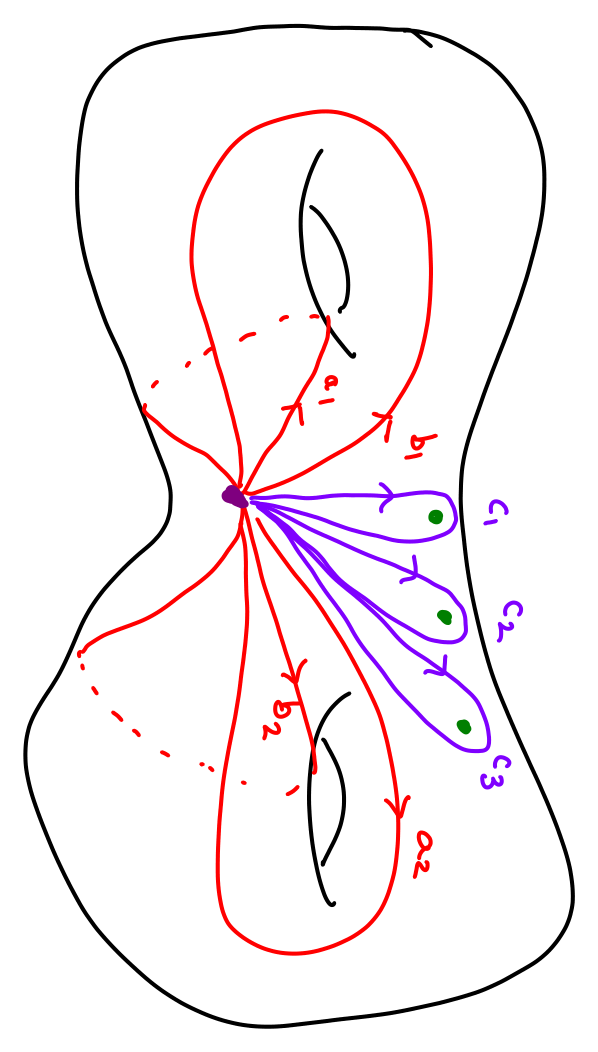
\includegraphics[width=0.6\textwidth]{figures/fig02.png}
  \caption{亏格为 2、带三个穿孔的曲面情形下，$\pi_1(\Sigma_2,x_0)$ 的一组生成元的选取。（原文 Fig.~2，第 35 页）}
  \label{fig:2}
\end{figure}

第二，在 $G$ 为阿贝尔、而 $X$ 任意的情形，同态 $\pi_1(X,x_0)\to G$ 通过同调上的一个同态分解：$H_1(X;\mathbb{Z})\to G$。这由 Stokes 定理可得：若 $\gamma-\gamma'=\partial\Sigma$，则\footnote{回忆我们的约定：当 $G$ 是环面群这一特殊情形时，我们把 $A$ 取作实形式。}

\begin{equation}
  \exp\Big[\mathrm{i}\oint_{\gamma}A\Big]\Big/\exp\Big[\mathrm{i}\oint_{\gamma'}A\Big]=\exp\Big[\mathrm{i}\int_{\Sigma}F\Big]=1
  \tag{2.112}
  \label{eq:2.112}
\end{equation}
事实上，这个论证表明：在阿贝尔情形，和乐只依赖于同调类 $[\gamma]\in H_1(\Sigma_2;\mathbb{Z})$。

于是，取 $G=U(1)$、$X=\Sigma_2$，我们便有

\begin{equation}
  \mathcal{M}_{\mathrm{flat}}=\operatorname{Hom}(H_1(\Sigma_2;\mathbb{Z}),U(1))
  \tag{2.113}
  \label{eq:2.113}
\end{equation}

现在 $\Sigma_2$ 的同调中没有挠元，故可以放心地说：

\begin{equation}
  \operatorname{Hom}(H_1(\Sigma_2;\mathbb{Z}),U(1))\cong H^{1}(\Sigma_2;\mathbb{R})/H^{1}(\Sigma_2;\mathbb{Z})
  \tag{2.114}
  \label{eq:2.114}
\end{equation}

这可以更直接地如下理解：我们可以直接解 $F=dA=0$。首先，这意味着第一 Chern 类为零，而它由 $\int_{\Sigma_2}F/2\pi=0$ 度量。

% [Tutor Note: (2.114) 用到两件事：一是泛系数定理给出 $\operatorname{Hom}(H_1(\Sigma_2;\mathbb{Z}),U(1))\cong H^1(\Sigma_2;\mathbb{Z})\otimes_{\mathbb{Z}}\mathbb{R}/\mathbb{Z}$，此处 $\Sigma_2$ 是闭曲面、同调无挠，故张量积与 $\operatorname{Hom}$ 一致；二是 $H^1(\Sigma_2;\mathbb{Z})\otimes\mathbb{R}\cong H^1(\Sigma_2;\mathbb{R})$。若换成带边或非紧的曲面，$H_1$ 的自由部分之外还要处理边界项，(2.113) 就不再是全部。另注意脚注 14 的实形式约定：$A$ 取实值，故 (2.116) 中 $\oint A$ 直接落在 $\mathbb{R}$ 上；若改用反厄米约定 $A\to-\mathrm{i}A$，则 (2.116)–(2.118) 的指数与系数都要相应补上 $\mathrm{i}$ 与 $2\pi$ 的因子。]

因此，我们可以把 $A$ 看成整体良定义的 1-形式。由于 $dA=0$，它是闭 1-形式。但我们必须商去平移 $A\to A+\omega$，其中 $\omega\in\Omega^{1}_{2\pi\mathbb{Z}}(\Sigma_2)$。所得空间就是

\begin{figure}[htbp]
  \centering
  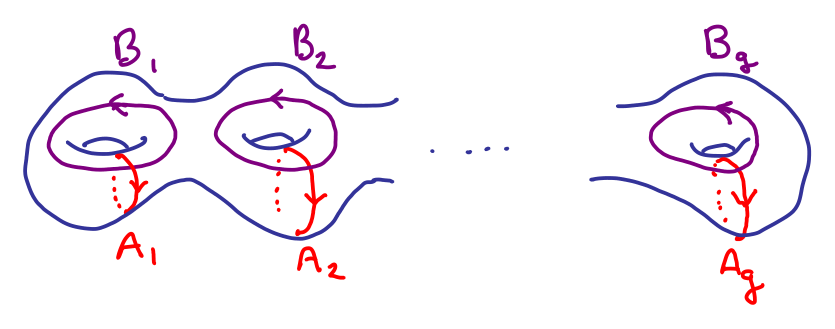
\includegraphics[width=0.55\textwidth]{figures/fig03.png}
  \caption{亏格为 $g$ 的曲面同调的一组标准基：该曲面以把手体（handlebody）表面的方式给出。（原文 Fig.~3，第 36 页；原文图注此行缺右括号，此处补全）}
  \label{fig:3}
\end{figure}

\begin{equation}
  \mathcal{M}_{\mathrm{flat}}=H^{1}(\Sigma_2;\mathbb{R})/H^{1}(\Sigma_2;\mathbb{Z})
  \tag{2.115}
  \label{eq:2.115}
\end{equation}

% 原文 (2.115) 的下标印作斜体 $flat$（(2.107)、(2.111)、(2.113)、(2.114)、(2.126) 则印作正体 $\mathrm{flat}$）；为片段内部统一，此处一律用 \mathrm{flat}。

这不过是一个 $2g$ 维的环面。若我们为同调选取显式的生成元 $A_I,B_I$（例如像图~\ref{fig:3} 那样），则有坐标

\begin{equation}
  e^{\mathrm{i}\theta_I}=e^{\mathrm{i}\oint_{A_I}A}
  \qquad\qquad
  e^{\mathrm{i}\phi_I}=e^{\mathrm{i}\oint_{B_I}A}
  \tag{2.116}
  \label{eq:2.116}
\end{equation}

在这些坐标下可以写出

\begin{equation}
  A=\theta_I\alpha_I+\phi_I\beta_I
  \tag{2.117}
  \label{eq:2.117}
\end{equation}

其中 $\alpha_I,\beta_I$ 是一次上同调类的一组对偶基，而

\begin{equation}
  \omega=\frac{\kappa}{\pi}\delta\theta_I\wedge\delta\phi_I
  \tag{2.118}
  \label{eq:2.118}
\end{equation}

% [Tutor Note: (2.118) 出现 $\kappa/\pi$ 而非环面公式里更眼熟的 $\kappa/2\pi$，原因有二：其一，辛形式取自 $\frac{\kappa}{2\pi}\int_{\Sigma_2}\delta A\wedge\delta A$，而 (2.117) 给出 $\int_{\Sigma_2}\delta A\wedge\delta A=2\,\delta\theta_I\wedge\delta\phi_I$（$\int_{A_J}\alpha_I=\delta_{IJ}$、$\int_{B_J}\beta_I=\delta_{IJ}$），因子 $2$ 把 $2\pi$ 抵消成 $\pi$；其二，$\theta_I,\phi_I$ 由 (2.116) 的 $e^{\mathrm{i}\theta_I}$ 定义，本身已是模 $2\pi$ 的坐标。用 $\{\theta_I,\phi_J\}=\frac{\pi}{\kappa}\delta_{IJ}$ 反推即可自查。另：(2.117)、(2.118) 中重复指标 $I$ 按 Einstein 约定求和，原文未显式写出 $\sum_I$。]

\textbf{注记：}

\begin{enumerate}
  \item \underline{维数公式}。警觉的读者会注意到，\eqref{eq:2.111} 有时可以是负的。确实，这是一个虚维数公式。若共轭作用在 $\operatorname{Hom}(\pi_1,G)$ 的光滑点处自由作用，它才真正给出某个流形的维数。然而，若群作用不是有效的，真实维数就不由该公式给出（如果那里还有个流形的话）。例如，考虑 $\Sigma_2$ 是不带穿孔的 $S^{2}$ 的情形。此时 $\pi_1$ 是只有一个元素的群，同态也只有一个。模叠就是叠 $pt//G$，形式上具有负维数。在接下来的几节中我们将研究 $G=U(1)$ 的环面。此时对易子方程事实上不施加任何约束，而共轭作用平凡地作用。所以真实维数是

  \begin{equation}
    2g\dim G=2\times 1\times 1=2
    \tag{2.119}
    \label{eq:2.119}
  \end{equation}

  而两个形式上的减法 $-\dim G-\dim G$ 对虚维数贡献 $-2$，也就是零。某种意义上每一点都是「奇异的」，因为除以共轭作用这件事处处都是平凡的。

  \item \underline{辛结构的内禀定义}。我们已经从 \eqref{eq:2.93} 看到，$\Sigma_2$ 上平坦规范场的空间是某个辛空间的 Hamilton 约化，因此辛形式继承自 \eqref{eq:2.79}。在阿贝尔情形把它写下来相当直接，正如我们上面所做的。在非阿贝尔情形，写出显式公式则更具挑战性。这件事在 [24, 25] 中完成了，我们这里给出简要描述。记 $\pi:=\pi_1(\Sigma_2,x_0)$。设有同态 $\phi:\pi\to G$。通过在 $\phi$ 处构造同态空间的一个切向量 $v$，人们容易看出 $v$ 应被视为一个群上循环 $\phi\in Z^{1}(\pi;\mathfrak{g}_{\mathrm{Ad}(\phi)})$。这里我们用的是系数取自 $\pi$ 的某个表示中的群上循环，该表示由 $\rho(\gamma):=\mathrm{Ad}(\phi(\gamma))$ 作用在 $\mathfrak{g}$ 上给出。为了理解这一点，设有同态族 $\phi_t:\pi\to G$，它给出在 $t=0$ 时刻经过 $\phi=\phi_0$ 的一条路径。那么，对每个 $\gamma\in\pi$ 我们都有 $G$ 中群元素的一条路径：$\phi_t(\gamma)=g_\gamma(t)$。现在定义

  \begin{equation}
    v:\pi\to\mathfrak{g}
    \tag{2.120}
    \label{eq:2.120}
  \end{equation}

  为

  \begin{equation}
    v(\gamma):=\phi(\gamma)^{-1}\frac{d}{dt}\Big|_{0}\phi_t(\gamma)=g_\gamma(0)^{-1}\frac{d}{dt}\Big|_{0}g_\gamma(t)
    \tag{2.121}
    \label{eq:2.121}
  \end{equation}

  现在我们必须施加群同态性质：

  \begin{equation}
    \phi_t(\gamma_1)\phi_t(\gamma_2)=\phi_t(\gamma_1\gamma_2)
    \tag{2.122}
    \label{eq:2.122}
  \end{equation}

  它对一切 $\gamma_1,\gamma_2\in\pi$ 成立。在 $t=0$ 处求导，并把方程左乘 $\phi_0(\gamma_1\gamma_2)^{-1}$，得到：

  \begin{equation}
    \mathrm{Ad}(\phi_0(\gamma_2))v(\gamma_1)-v(\gamma_1\gamma_2)+v(\gamma_2)=0
    \tag{2.123}
    \label{eq:2.123}
  \end{equation}
\end{enumerate}

% 跨片段引用说明：\eqref{eq:2.93} 与 \eqref{eq:2.79} 指向 c03 片段中的 (2.93)、(2.79)（平坦联络空间作为辛空间的 Hamilton 约化），其 \label 由 c03 提供，本片段不重复引入。

% [Tutor Note: 第 2 条注记里「one easily sees that $v$ should be considered as a group cocycle」这一步的实质是把「同态空间在 $\phi$ 处的切向量」认同为 $\pi$ 的 1-上循环；原文这里把上循环也记作 $\phi$（应为 $v$），与同态本身重名，读者须按 (2.121) 的定义把 $v$ 与 $\phi$ 区分开。真正的计算在 (2.122)$\to$(2.123)：对 $\phi_t(\gamma_1)\phi_t(\gamma_2)=\phi_t(\gamma_1\gamma_2)$ 求导得 $\dot\phi_t(\gamma_1)\phi_t(\gamma_2)+\phi_t(\gamma_1)\dot\phi_t(\gamma_2)=\dot\phi_t(\gamma_1\gamma_2)$，再用 $\phi_t(\gamma_1)^{-1}\dot\phi_t(\gamma_1)=v(\gamma_1)$ 把各项都化成 $v$，才得到 (2.123) 的三项式。]

这正是系数取在 $\mathfrak{g}$ 中的群上循环条件，其中 $\mathfrak{g}$ 通过 $\gamma\to\mathrm{Ad}(\phi(\gamma))$ 被看作一个 $\pi$-表示。这种上循环构成的空间记作 $Z^{1}(\pi;\mathfrak{g}_{\mathrm{Ad}(\phi)})$。另一方面，若作一族同态

\begin{equation}
  \phi_t(\gamma)=g(t)^{-1}\phi(\gamma)g(t)
  \tag{2.124}
  \label{eq:2.124}
\end{equation}

其中 $g(t)=e^{-tX}$ 是某一族，$X\in\mathfrak{g}$，那么由于我们的空间是商去 $G$ 的共轭作用而得到的，显然应当模去这类切向量。再次在 $t=0$ 处求导可知，这类切向量是

\begin{equation}
  v(\gamma)=\mathrm{Ad}(\phi(\gamma))X-X
  \tag{2.125}
  \label{eq:2.125}
\end{equation}

这正是一边上循环 $B^{1}(\pi;\mathfrak{g}_{\mathrm{Ad}(\phi)})$ 的定义。于是我们断定，存在自然的同构

\begin{equation}
  T_{[\phi]}\mathcal{M}_{\mathrm{flat}}\cong H^{1}(\pi;\mathfrak{g}_{\mathrm{Ad}(\phi)})
  \tag{2.126}
  \label{eq:2.126}
\end{equation}

现在，由于 $\Sigma_2$ 有单连通的覆叠\footnote{这就是单值化定理（uniformization theorem）：$g=0$ 时它单连通，$g=1$ 时覆叠是 $\mathbb{C}$，$>1$ 时则是上半平面，或等价地是圆盘。技术上，我们所用的条件是：只要 $\Sigma_2$ 不是不带穿孔的球面，该曲面就是 $K(\pi,1)$ 空间。}，我们可以把群上同调与奇异上同调等同起来：$H^{k}(\pi;M)\cong H^{k}(\Sigma_2;M)$。确实，若我们有平坦 $G$ 丛 $P\to\Sigma_2$，则存在伴随丛，而平坦 $G$ 丛的空间在某点的切空间是 $H^{1}(\Sigma_2;\mathrm{ad}P)$。利用 $\mathfrak{g}$ 上的迹形式，相乘并积分，我们便得到一个映射

\begin{equation}
  H^{1}(\pi;\mathfrak{g}_{\mathrm{Ad}(\phi)})\times H^{1}(\pi;\mathfrak{g}_{\mathrm{Ad}(\phi)})\to\mathbb{R}
  \tag{2.127}
  \label{eq:2.127}
\end{equation}

这就是辛形式的 Goldman 描述。描述它的一个有用方式，是用经典 Wilson 线的 Poisson 括号。一般地，若 $f:G\to\mathbb{R}$ 是 $\mathrm{Ad}$-不变函数，令 $df:G\to\mathfrak{g}$ 为由下式定义的函数

\begin{equation}
  \frac{d}{dt}\Big|_{0}f(ge^{tX})=\operatorname{tr}\big(df(g)X\big)
  \tag{2.128}
  \label{eq:2.128}
\end{equation}

那么 [25] 中证明了：若 $W_R(\gamma,A)=\operatorname{Tr}_R P\exp\oint_{\gamma}A$，则可以为这些函数的 Poisson 括号写出一个漂亮的显式公式：

\begin{equation}
  \{W_R([\gamma_1],\cdot),W_R([\gamma_2],\cdot)\}
  =\sum_{p\in\gamma_1\cap\gamma_2}\iota_p(\gamma_1,\gamma_2)\operatorname{tr}\big(dW_R(\gamma_1(p),\cdot)\,dW_R(\gamma_2(p),\cdot)\big)
  \tag{2.129}
  \label{eq:2.129}
\end{equation}

在这个公式中，我们为同伦类选取了在有限多个点上横截相交的一般位置代表元 $\gamma_1,\gamma_2$。对 $p\in\gamma_1\cap\gamma_2$，我们用 $\gamma_i(p)$ 记 $\gamma_i$ 的以 $p$ 为基点的代表元。这并不显然，但确实右端所用的代表元的选取无关紧要。

考虑到规范场上 (3.38) 的 Poisson 括号，括号 \eqref{eq:2.129} 是非常合理的：delta 函数的支集意味着只可能有来自交点的贡献。然后作一个简单的局部分析，就可以推出该公式。

% 跨片段引用：正文中的 (3.38) 指第 3 章给出的规范场 Poisson 括号（该章片段尚未译出），此处按原文以文字标注编号，待第 3 章片段就位后可改用 \eqref{eq:3.38}。

{\small\itshape ［原文标记：这件事应当详细做一遍！！本质上这正是 GMN2 的附录 B 中所做的事。］}% [原文待办标记，原文 p.38 右边栏]

% [Tutor Note: (2.129) 中「It is not obvious, but it is true that the choice of representative used on the RHS does not matter」省略的论证是：改换代表元 $\gamma_i\mapsto\eta_i^{-1}\gamma_i\eta_i$（$\eta_i$ 基于交点 $p$）只使 $dW_R$ 在 $\gamma_i(p)$ 处共轭，而 $\operatorname{tr}$ 循环不变，故右端不变；同时交点数 $\iota_p(\gamma_1,\gamma_2)=\pm1$ 的符号依赖于曲面定向与 $\gamma_1,\gamma_2$ 在 $p$ 处有序切向的夹角方向，换定向会使整个括号变号——这与 $\{\cdot,\cdot\}$ 作为辛形式之逆的定义是自洽的。原文未交代 $\iota_p$ 的符号约定，核对时须与本段的辛形式 (2.118) 定向一致。]
